\chapter{Metodologia}

Na Figura \ref{fig:metodologia} é ilustrado em fluxograma as etapas citadas neste capítulo para desenvolvimento do trabalho.

\begin{figure}[H]
    \centering
    \caption{Fluxograma das etapas executadas na metodologia}
    % 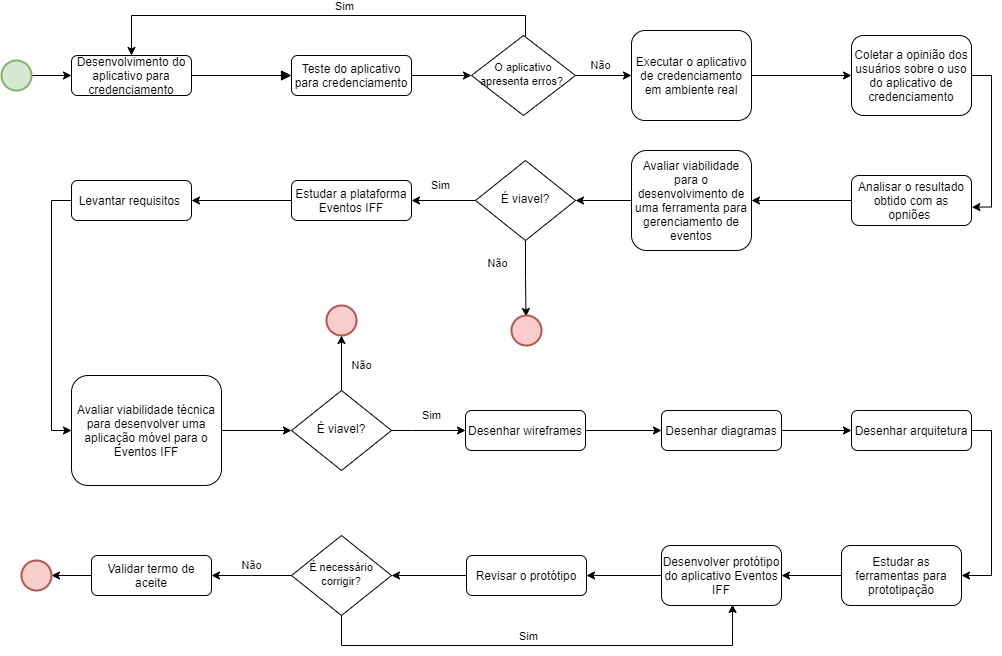
\includegraphics[scale=0.45]{figuras/metodologia.jpg}
    \fbox{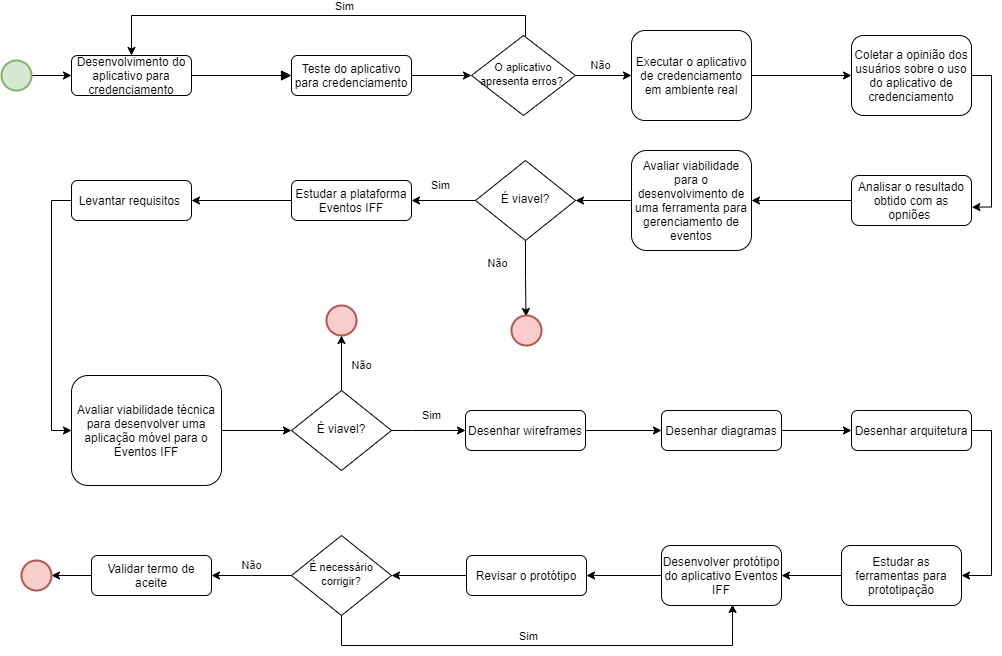
\includegraphics[scale=0.43]{figuras/metodologia.jpg}}
    \label{fig:metodologia}
    \legend{Fonte: elaborado pelos autores}
\end{figure}

Esse trabalho foi desenvolvido seguindo as seguintes etapas, nas respectivas ordens: 

\begin{enumerate}
  \item Desenvolvimento de um aplicativo para validação da funcionalidade de credenciamento;
  \item Testes do aplicativo: nessa etapa é realizado testes executados pelos desenvolvedores para validação;
  \item Execução do aplicativo em ambiente real: o aplicativo é disponibilizado para uso no evento Congresso Integrado da Tecnologia da Informação (CITI) 2019;
  \item Coleta das opiniões dos usuários do aplicativo através de formulário;
  \item Análise do resultado obtido com o formulário de opinião;
  \item Avaliação da viabilidade da ferramenta para credenciamento em eventos acadêmicos;
  \item Estudo da plataforma \textit{web} Eventos IFF;
  \item Levantamento de requisitos para desenvolvimento do aplicativo móvel para o Eventos IFF;
  \item Avaliação da viabilidade técnica de implementação e integração de uma ferramenta móvel para a plataforma Eventos IFF;
  \item Desenho de \textit{wireframes} das funcionalidades levantadas com a análise de requisitos;
  \item Desenho dos diagramas de caso de uso e de classe;
  \item Desenho da arquitetura da solução;
  \item Estudo das ferramentas existentes para prototipação;
  \item Desenvolvimento do protótipo na plataforma selecionada;
  \item Revisão e correção do protótipo;
  \item Termo de aceite do protótipo.
\end{enumerate}